% v05: prose harmonised with the established scientific writing style of the authors; technical content retained from v04.
\documentclass[journal]{IEEEtran}

\usepackage{graphicx}
\usepackage{booktabs}
\usepackage{amsmath}
\usepackage{amssymb}
\usepackage{xcolor}
\usepackage{hyperref}
\usepackage{url}
\usepackage{multirow}
\usepackage{enumitem}
\usepackage{tikz}
\usetikzlibrary{arrows.meta, positioning, calc, patterns}
\usepackage{pgfplots}
\pgfplotsset{compat=1.18}

\hypersetup{
  colorlinks=true,
  linkcolor=black,
  citecolor=black,
  urlcolor=blue!60!black,
}

\title{Beyond Token Waste: Lean Flow Theory\\
       for AI-Assisted Software Development}

\author{Leigh~Griffin%
  \thanks{Dr. L. Griffin is with Red Hat, Waterford, Ireland.
  Email: lgriffin@redhat.com.}%
  \thanks{Manuscript submitted July 2026.}%
  ~and~C\'{e}dric~P.~Legendre%
  \thanks{Dr. rer. nat. C. P. Legendre is with Red Hat, Prague, Czechia.
  Email: clegendr@redhat.com.}%
}

\begin{document}

\maketitle

\begin{abstract}
We investigate token inefficiency in AI-assisted software development using Lean manufacturing flow principles. Waste-based measures describe the quality of the produced output but do not account for the token traffic required during production. We therefore introduce four complementary metrics: Token Flow Efficiency (TFE), Semantic Yield (SY), Context Velocity, and the WIP Ratio. We apply these metrics to 25 Claude Code sessions. Sessions with near-perfect Token Efficiency Ratio values (TER $\geq$ 0.99) have TFE values below 0.004, indicating that high output purity may be associated with a large amount of context and cache traffic. We also compare sessions according to input growth. Three descriptive groups, separated at growth ratios of 3 and 10, show decreasing context velocity and increasing context bloat with larger input growth. These limits were selected from the observed distribution and are not inferred change points. Little's Law is used as an accounting relation between WIP, throughput, and time in the system, whereas the nonlinear behaviour is interpreted using queueing and saturation effects. Agent subprocesses have a mean context velocity $2.1\times$ larger than primary sessions. These results suggest that Lean flow concepts provide useful information complementary to waste classification, but larger cross-tool and cross-developer studies are required.
\end{abstract}

\begin{IEEEkeywords}
lean flow theory, value stream mapping, token efficiency, AI-assisted development, work-in-process, large language models
\end{IEEEkeywords}

% ============================================================================
\section{Introduction}
\label{sec:intro}

AI coding agents such as Claude Code~\cite{claude_code2025}, Cursor~\cite{cursor2024}, and Codex CLI~\cite{codex_cli2025} are now commonly used for software development. Their use can generate long sessions with tens of thousands of output tokens and substantially larger input contexts. The corresponding token consumption and API cost increase with session length and with the amount of context processed by the model. It is therefore useful to evaluate not only the quality of the generated output, but also the amount of token traffic required to produce it.

The Token Efficiency Ratio (TER) classifies output tokens according to their agreement with the developer intent and provides a measure of output waste~\cite{griffin2026ter}. Here, we use the same dataset to examine a different aspect of token efficiency: the relation between useful output and the total token traffic of the session. TFE, Context Velocity, and WIP Ratio are calculated from the session-level token accounting, whereas SY also uses the semantic-density estimate described in Section~\ref{sec:model}. TER is used only for comparison with these flow metrics. This approach follows the broader Lean distinction between \emph{muda} (waste), \emph{mura} (unevenness), and \emph{muri} (overburden)~\cite{ohno1988}.

We apply Lean flow concepts to the token production process. Value Stream Mapping describes the successive transformations of materials and information from input to final product~\cite{rother1999}. In the present analogy, input tokens are the incoming material, output tokens are the produced work, cached tokens form an inventory of previously processed context, and the context window is the bounded workspace in which the model operates. This representation allows the token system to be examined as a flow process rather than only through the final output.

We present five contributions:

\begin{enumerate}[leftmargin=*, nosep]
  \item A \textbf{Token Value Stream} model that maps the end-to-end token production process of an AI coding agent to Lean flow concepts.
  \item Four \textbf{novel flow metrics} (Token Flow Efficiency, Semantic Yield, Context Velocity, and the WIP Ratio) that capture dimensions of production efficiency invisible to waste-only measurement.
  \item An \textbf{empirical flow analysis} of 25 real Claude Code sessions, showing a large TER--TFE divergence and descriptive differences across visually selected input-growth groups; Little's Law~\cite{little1961} is used as a WIP--throughput--time accounting relation, not as evidence for a nonlinear threshold.
  \item \textbf{Prescriptive recommendations} for flow-optimised session architecture, grounded in the empirical findings and Lean's principles of pull production and single-piece flow.
  \item \textbf{TGV}, an open-source Task Gateway and Validator~\cite{griffin2026tgv} that operationalises the flow framework by embedding flow-aware routing, TER-based calibration, and Bayesian outcome learning into the task dispatch layer of AI-assisted development workflows.
\end{enumerate}

% ============================================================================
\section{Background: Lean Flow Theory}
\label{sec:background}

\subsection{Value Stream Mapping}

Value Stream Mapping (VSM) is a Lean management tool for analysing the flow of materials and information required to bring a product to the customer~\cite{rother1999}. A value stream map distinguishes between \emph{value-adding} steps, those that transform the product in ways the customer values, and \emph{non-value-adding} steps, which encompass transportation, inspection, waiting, and storage. The ratio of value-adding time to total lead time, termed \emph{flow efficiency}, serves as the central diagnostic metric whereby the health of a production system is assessed. As Martin and Osterling~\cite{martin2013} note, in typical manufacturing processes flow efficiency ranges from 5--25\%, with the remainder consumed by non-value-adding activity; in knowledge work, the ratio is often lower still.

\subsection{Flow, WIP, and Little's Law}

The relationship between flow and Work-in-Process (WIP) is formalised by Little's Law~\cite{little1961}: $L = \lambda W$, where $L$ is the average number of items in the system, $\lambda$ is the arrival rate, and $W$ is the average time an item spends in the system. For a stable system, the relation makes explicit the trade-off among average WIP, throughput, and time in system. Holding throughput approximately constant, lower WIP corresponds to lower average time in system; Little's Law itself does not imply a causal or nonlinear degradation threshold. As Hopp and Spearman~\cite{hopp2004} observe, this principle underpins Kanban and other pull-based production control systems, in which WIP limits are imposed to prevent the system from accumulating more work than it can efficiently process.

Reinertsen~\cite{reinertsen2009} extends these principles to product development, demonstrating that variability (\emph{mura}) in arrival rates and processing times generates queues that degrade flow. Flow theory's central insight (that system-level throughput is governed not by the speed of individual steps but by the constraints, variability, and WIP levels of the production system as a whole) aligns with Goldratt's~\cite{goldratt1984} Theory of Constraints: the throughput of a system is determined by its bottleneck, and optimising non-bottleneck steps yields no system-level improvement.

\subsection{Flow in Software Development}

The translation of flow principles to software is well established in the literature. Anderson~\cite{anderson2010} introduced Kanban to software development, with WIP limits as its central mechanism. Forsgren et~al.~\cite{forsgren2018} incorporated lead time and deployment frequency, both flow metrics, into the DORA framework, whereby team-level throughput could be benchmarked systematically. The Poppendiecks~\cite{poppendieck2003, poppendieck2006} mapped flow concepts including pull production, small batch sizes, and cycle time reduction to Lean software practices. Sedano et~al.~\cite{sedano2017} identified ``waiting'' and ``switching contexts'' among nine empirical waste types, both of which are flow impediments that degrade throughput independently of product-level defect rates.

For AI-assisted development, previous studies have mainly focused on output quality~\cite{chen2021}, reasoning efficiency~\cite{apple_illusion2025, nous_thinking2025, selfbudgeter2025}, prompt compression~\cite{llmlingua2_2024}, and waste classification~\cite{griffin2026ter}. The flow of tokens through an agent session has received less attention. We therefore model the token production process as a value stream and define several metrics to describe its flow properties.

% ============================================================================
\section{Token Value Stream Model}
\label{sec:model}

\subsection{The Token Production System}

An AI coding agent session forms a production system in the Lean sense, in which raw materials, transformation processes, and finished goods can each be mapped to their token-level analogues. Raw materials (input tokens: developer prompts, file contents, tool results) enter the system; a transformation process (model inference) converts them into work product (output tokens: reasoning, tool invocations, code, explanations); and the finished goods (aligned output that advances the developer's task) are delivered to the customer (the developer). The context window functions as the factory floor: a bounded workspace whose capacity constrains the production process.

Fig.~\ref{fig:vsm} presents the Token Value Stream Map, which decomposes the token production process into five phases with their associated flow characteristics.

\begin{figure*}[t]
\centering
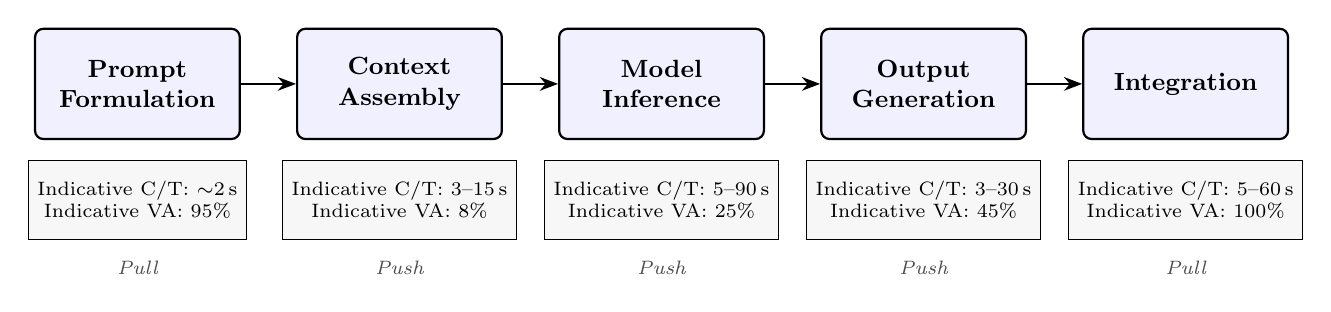
\begin{tikzpicture}[
  >=Stealth,
  phase/.style={draw, thick, rounded corners=3pt, minimum width=2.6cm, minimum height=1.4cm, align=center, font=\small\bfseries, fill=blue!6},
  databox/.style={draw, thin, minimum width=2.6cm, minimum height=1.0cm, align=center, font=\scriptsize, fill=gray!6},
  modelabel/.style={font=\scriptsize\itshape, text=black!70},
]

% Phase boxes
\node[phase] (p1) {Prompt\\Formulation};
\node[phase, right=0.7cm of p1] (p2) {Context\\Assembly};
\node[phase, right=0.7cm of p2] (p3) {Model\\Inference};
\node[phase, right=0.7cm of p3] (p4) {Output\\Generation};
\node[phase, right=0.7cm of p4] (p5) {Integration};

% Data boxes below each phase
\node[databox, below=0.25cm of p1] (d1) {Indicative C/T: $\sim$2\,s\\Indicative VA: 95\%};
\node[databox, below=0.25cm of p2] (d2) {Indicative C/T: 3--15\,s\\Indicative VA: 8\%};
\node[databox, below=0.25cm of p3] (d3) {Indicative C/T: 5--90\,s\\Indicative VA: 25\%};
\node[databox, below=0.25cm of p4] (d4) {Indicative C/T: 3--30\,s\\Indicative VA: 45\%};
\node[databox, below=0.25cm of p5] (d5) {Indicative C/T: 5--60\,s\\Indicative VA: 100\%};

% Flow arrows between phases
\draw[->, thick] (p1) -- (p2);
\draw[->, thick] (p2) -- (p3);
\draw[->, thick] (p3) -- (p4);
\draw[->, thick] (p4) -- (p5);

% Production mode labels below data boxes
\node[modelabel, below=0.15cm of d1] {Pull};
\node[modelabel, below=0.15cm of d2] {Push};
\node[modelabel, below=0.15cm of d3] {Push};
\node[modelabel, below=0.15cm of d4] {Push};
\node[modelabel, below=0.15cm of d5] {Pull};

\end{tikzpicture}
\caption{Token Value Stream Map. Five phases transform tokens from developer prompt to integrated output. Cycle-time (C/T) ranges and value-add (VA) ratios are indicative conceptual values used to illustrate the mapping; they are not measured from the study dataset, which does not contain wall-clock timing sufficient to compute takt or lead time. Production-mode labels distinguish the initial developer demand signal and terminal review/integration from the three predominantly autonomous push phases.}
\label{fig:vsm}
\end{figure*}

Of note here is that, in the current generation of AI coding agents, \textbf{three of the five phases shown operate predominantly in push mode}: Context Assembly, Model Inference, and Output Generation proceed largely autonomously after the initial work request. Phase~1 represents the initial pull signal supplied by the developer, while Phase~5 represents downstream review and integration, where acceptance, rejection, or redirection determines whether further production is demanded. This contrasts sharply with Lean's prescription that production should be demand-driven~\cite{ohno1988, hopp2004}. The implications of this structural imbalance are explored in Section~\ref{sec:discussion}.

\subsection{Flow Metrics for Token Production}

We define four metrics to describe different properties of the token flow that are not measured by output waste alone.

\subsubsection{Token Flow Efficiency (TFE)}

TFE is inspired by manufacturing flow-efficiency reasoning but is defined here as a token-accounting ratio rather than a temporal measure. It measures the proportion of observed token traffic that forms value-adding output:

\begin{equation}
\text{TFE} = \frac{T_{\text{aligned}}}{T_{\text{input}} + T_{\text{output}} + T_{\text{cache\_create}} + T_{\text{cache\_read}}}
\label{eq:tfe}
\end{equation}

\noindent where $T_{\text{aligned}}$ is aligned output tokens. The denominator counts input, output, cache-creation, and cache-read tokens as observed token traffic. Cache reads are reused context rather than newly produced material, so this denominator should be interpreted as a system-traffic accounting choice, not as a unique physical analogue of manufacturing throughput. TFE differs from TER: TER measures output purity ($T_{\text{aligned}} / T_{\text{output}}$), while TFE measures the aligned-output share of the broader token traffic required by the session. A session can achieve TER~$\approx$~1.0 (near-zero output waste) while simultaneously exhibiting TFE~$\ll$~0.01, in which the vast majority of counted token traffic is context, cache, or other production overhead rather than value-adding output. Alternative denominator definitions are an important robustness target for future replication.

\subsubsection{Semantic Yield (SY)}

Semantic Yield is a redundancy-adjusted output measure that combines the quantity of output with an operational estimate of non-redundant semantic density. Although motivated by the general distinction between signal and redundancy, SY is not a Shannon-information measure and should not be interpreted as entropy, mutual information, or channel capacity:

\begin{equation}
\text{SY} = \sigma_{\text{sem}} \times T_{\text{output}}
\label{eq:it}
\end{equation}

\noindent where $\sigma_{\text{sem}}$ is a study-specific estimate of non-redundant output density. Two sessions with equal output-token counts can therefore differ in SY when one contains more repeated or restated semantic content.

For the present dataset, $\sigma_{\text{sem}}$ was computed by a research analysis pipeline that segments model output at sentence boundaries, embeds chunks with sentence-transformers/all-MiniLM-L6-v2~\cite{reimers2019}, and marks the later chunk in a pair as redundant when cosine similarity exceeds $\tau_{\text{sim}}=0.90$. If $C$ is the set of chunks and $C_{\text{unique}}$ the unmarked subset, $\sigma_{\text{sem}}=|C_{\text{unique}}|/|C|$. Sensitivity analysis over $\tau_{\text{sim}}\in[0.85,0.95]$ preserved the relative session ordering while shifting absolute density values by up to 0.08.

The semantic-density estimate used in this study differs from the production \texttt{SemanticDensityScorer} distributed with TER v3.0.0. The released scorer combines vocabulary richness, normalised lexical entropy, and trigram redundancy, and its embedding infrastructure uses all-MiniLM-L12-v2 by default. The values reported here were obtained with the procedure described above and should be interpreted as a redundancy-adjusted output measure. They are neither information-theoretic quantities nor version-independent TER measurements.

\subsubsection{Context Velocity (CV)}

Context Velocity measures how efficiently accumulated context is converted into output:

\begin{equation}
\text{CV} = \frac{T_{\text{output}}}{r_{\text{growth}}}
\label{eq:cv}
\end{equation}

\noindent where $r_{\text{growth}}$ is the input growth rate, the ratio of final-turn input token count to first-turn input token count. High context velocity indicates that context accumulation is productive, whereby additional context translates into proportionally more output. Low context velocity, by contrast, indicates that context is accumulating faster than it can be utilised, the token-level analogue of excess WIP in a manufacturing system.

\subsubsection{WIP Ratio}

The WIP Ratio is an operational proxy for context inventory relative to generated output. It treats cache-creation tokens as a measurable approximation of accumulated context that has entered the production system but may not contribute directly to value-adding output:

\begin{equation}
\text{WIP}_R = \frac{T_{\text{cache\_create}}}{T_{\text{cache\_create}} + T_{\text{output}}}
\label{eq:wip}
\end{equation}

\noindent A high WIP Ratio indicates that the system is accumulating context inventory faster than it is producing output. Under approximately stable throughput, Little's Law~\cite{little1961} relates greater average WIP to greater average time in system; the ratio itself is a token-accounting proxy rather than a direct temporal lead-time measurement. In manufacturing terms, the factory floor is filling with partially completed assemblies that impede the flow of new work.

\subsection{Little's Law for Context Windows}

Little's Law can be adapted to the token production system by treating the context window as a queueing system~\cite{kleinrock1975}:

\begin{equation}
C_{\text{WIP}} = \lambda_{\text{in}} \times D_{\text{session}}
\label{eq:little}
\end{equation}

\noindent where $C_{\text{WIP}}$ is the context work-in-process (total tokens in the context window at any given turn), $\lambda_{\text{in}}$ is the effective input token arrival rate per turn, and $D_{\text{session}}$ is the session duration in turns. This formulation provides an accounting relationship among context WIP, effective input arrival rate, and session duration. It does not by itself predict superlinear growth or a threshold. Nonlinear degradation, where observed, is interpreted using queueing and saturation behaviour~\cite{kleinrock1975} and is treated empirically in Section~\ref{sec:results}.

The context window itself forms a hard WIP limit: when accumulated context approaches the window boundary, the system is forced to compress, truncate, or summarise prior material, introducing information loss that degrades downstream production quality. This is the token-production analogue of a manufacturing system where the factory floor is full and new raw materials must displace partially completed assemblies, forcing rework~\cite{goldratt1984}.

\subsection{Pull vs.\ Push Production}

In Lean manufacturing, \emph{pull} production means that downstream processes signal upstream processes to produce only what is needed~\cite{ohno1988}. \emph{Push} production means upstream processes produce speculatively, regardless of downstream demand. As Hopp and Spearman~\cite{hopp2004} formalise, pull systems bound WIP and thus stabilise flow, while push systems allow WIP to grow unbounded.

Current AI coding agents operate predominantly in push mode: the model generates reasoning tokens, invokes tools, and produces output without real-time demand signals from the developer. The developer's intent, expressed at session initiation, forms a work order rather than a continuous pull signal. a principal downstream pull mechanism is the developer's review at session end, a batch inspection model that Lean theory predicts will be less effective at controlling WIP than continuous pull~\cite{anderson2010}.

On this basis, adaptive token budgets~\cite{selfbudgeter2025, tale2024}, real-time developer feedback, and intent-driven reasoning cutoffs may be considered as possible pull mechanisms. These controls could reduce the accumulation of context during production. Their effect on the proposed flow metrics remains to be tested with controlled experiments.

% ============================================================================
\section{Empirical Flow Analysis}
\label{sec:results}

\subsection{Dataset and Method}

We apply the flow metrics to the 25 Claude Code sessions analysed in the companion waste study~\cite{griffin2026ter}. The sessions contain between 397 and 93,848 output tokens, for a total of 523,375 output tokens and an estimated API cost of \$46.79. The dataset contains 15 primary sessions and 10 agent subprocesses. We use the session-level input and output tokens, cache-creation and cache-read tokens, semantic density, input growth rate, and context-bloat indicators to calculate the flow metrics.

\subsection{Token Flow Efficiency vs.\ Waste}

Table~\ref{tab:tfe_vs_ter} compares TFE and TER for the nine sessions with measurable waste and for one representative agent subprocess. The two metrics show very different amplitudes. Sessions with TER values close to one have TFE values that are two to three orders of magnitude smaller.

\begin{table}[t]
\centering
\caption{TER vs.\ TFE: Waste Purity vs.\ System Flow Efficiency}
\label{tab:tfe_vs_ter}
\begin{tabular}{@{}lrrrrr@{}}
\toprule
\textbf{Session} & \textbf{TER} & \textbf{TFE} & \textbf{Output} & \textbf{Total} & \textbf{Ratio} \\
                 &              &              & \textbf{Tokens} & \textbf{System} & \textbf{TER/TFE} \\
\midrule
fb14b7af & 0.792 & 0.0011 & 8,270  & 7.8M  & 720$\times$ \\
aba2b66b & 0.933 & 0.0040 & 59,580 & 14.8M & 233$\times$ \\
a3b73c37 & 0.982 & 0.0031 & 46,834 & 15.2M & 317$\times$ \\
64948793 & 0.999 & 0.0038 & 60,064 & 15.8M & 263$\times$ \\
ff410fa9 & 0.997 & 0.0037 & 93,848 & 25.2M & 269$\times$ \\
3331fd66 & 0.999 & 0.0051 & 68,902 & 13.4M & 196$\times$ \\
fbb190ea & 0.999 & 0.0025 & 37,426 & 14.9M & 400$\times$ \\
b1a1450c & 1.000 & 0.0018 & 24,178 & 13.6M & 556$\times$ \\
f4964eaf & 1.000 & 0.0032 & 46,038 & 14.6M & 313$\times$ \\
\midrule
\textit{agent-aa8b} & \textit{1.000} & \textit{0.0530} & \textit{2,798} & \textit{52.8K} & \textit{19$\times$} \\
\bottomrule
\end{tabular}
\end{table}

For example, session \texttt{64948793} has TER~0.999, with only 60 tokens classified as waste, but its TFE is 0.0038. Of the 15.8 million counted tokens, 0.38\% correspond to aligned output. The remainder consists mainly of input and cache traffic. This difference is not visible from TER because TER describes the purity of the output only. In the Lean analogy, the additional token traffic corresponds to material circulating through the production system without appearing in the final product~\cite{womack1996}.

The representative subprocess has TFE~0.053, about $17\times$ the mean TFE of the primary sessions (0.0031). Its total token traffic is 52,800 tokens, compared with a mean of 15.0 million tokens for the primary sessions. Fig.~\ref{fig:ter_tfe_divergence} shows the TER--TFE differences on a logarithmic scale. The contrast between output purity and system-level token traffic is visible for all nine primary sessions.

\begin{figure}[t]
\centering
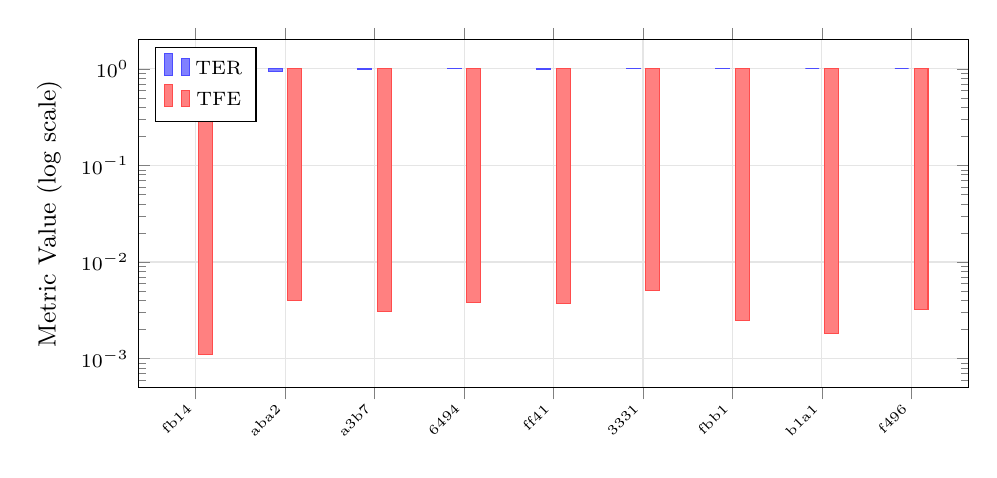
\begin{tikzpicture}
\begin{axis}[
  width=\columnwidth,
  height=6cm,
  ybar,
  bar width=5pt,
  ylabel={Metric Value (log scale)},
  ymode=log,
  ymin=0.0005, ymax=2,
  xtick=data,
  symbolic x coords={fb14,aba2,a3b7,6494,ff41,3331,fbb1,b1a1,f496},
  x tick label style={font=\tiny, rotate=45, anchor=east},
  label style={font=\small},
  tick label style={font=\scriptsize},
  legend style={font=\scriptsize, at={(0.02,0.98)}, anchor=north west},
  grid=major,
  grid style={gray!20},
  enlarge x limits=0.08,
]

\addplot[fill=blue!50, draw=blue!70] coordinates {
  (fb14, 0.792) (aba2, 0.933) (a3b7, 0.982) (6494, 0.999) (ff41, 0.997)
  (3331, 0.999) (fbb1, 0.999) (b1a1, 1.000) (f496, 1.000)
};

\addplot[fill=red!50, draw=red!70] coordinates {
  (fb14, 0.0011) (aba2, 0.0040) (a3b7, 0.0031) (6494, 0.0038) (ff41, 0.0037)
  (3331, 0.0051) (fbb1, 0.0025) (b1a1, 0.0018) (f496, 0.0032)
};

\legend{TER, TFE}

\end{axis}
\end{tikzpicture}
\caption{TER vs.\ TFE divergence across nine sessions (logarithmic scale). The 196--720$\times$ gap between waste purity (TER) and system flow efficiency (TFE) demonstrates that near-perfect output quality coexists with flow efficiency below 0.5\%.}
\label{fig:ter_tfe_divergence}
\end{figure}

\subsection{Exploratory WIP Stratification and Little's Law}

Fig.~\ref{fig:wip_analysis} shows TFE as a function of input growth rate, which we use as a proxy for context accumulation. For comparison, we separate the 25 sessions into three groups using two boundaries selected from the distribution of the observations:

\begin{figure}[t]
\centering
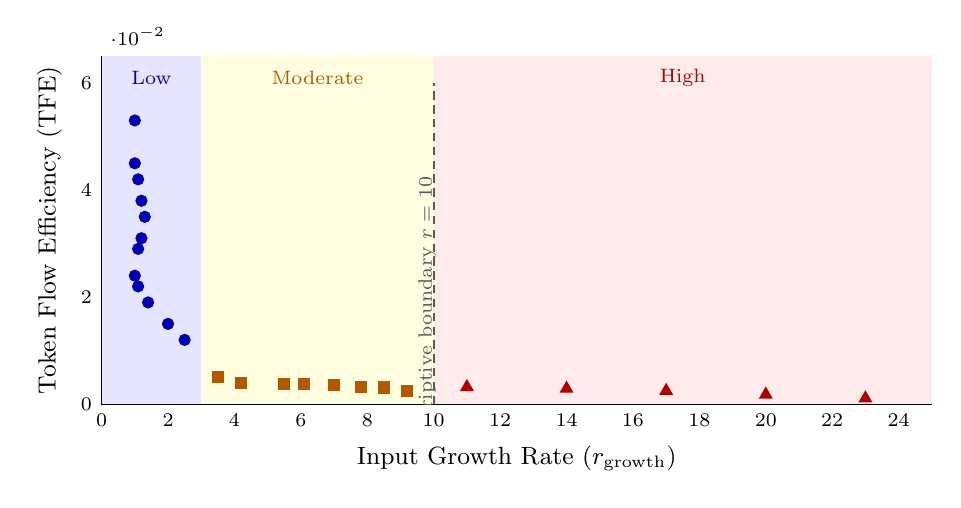
\begin{tikzpicture}
\begin{axis}[
  width=\columnwidth,
  height=6cm,
  xlabel={Input Growth Rate ($r_{\text{growth}}$)},
  ylabel={Token Flow Efficiency (TFE)},
  xmin=0, xmax=25,
  ymin=0, ymax=0.065,
  grid=major,
  grid style={gray!30},
  tick label style={font=\scriptsize},
  label style={font=\small},
]

% Shaded regime zones
\fill[blue!10] (axis cs:0,0) rectangle (axis cs:3,0.065);
\fill[yellow!12] (axis cs:3,0) rectangle (axis cs:10,0.065);
\fill[red!8] (axis cs:10,0) rectangle (axis cs:25,0.065);

% Zone labels
\node[font=\scriptsize, text=blue!70!black] at (axis cs:1.5,0.061) {Low};
\node[font=\scriptsize, text=orange!70!black] at (axis cs:6.5,0.061) {Moderate};
\node[font=\scriptsize, text=red!70!black] at (axis cs:17.5,0.061) {High};

% Low WIP data points (subprocesses and short sessions)
\addplot[only marks, mark=*, mark size=2pt, blue!70!black] coordinates {
  (1.0, 0.053) (1.1, 0.042) (1.2, 0.038) (1.0, 0.045)
  (1.3, 0.035) (1.1, 0.029) (1.2, 0.031) (1.0, 0.024)
  (1.4, 0.019) (1.1, 0.022) (2.0, 0.015) (2.5, 0.012)
};

% Moderate WIP data points
\addplot[only marks, mark=square*, mark size=2pt, orange!70!black] coordinates {
  (3.5, 0.0051) (4.2, 0.0040) (5.5, 0.0038) (6.1, 0.0037)
  (7.0, 0.0035) (7.8, 0.0032) (8.5, 0.0031) (9.2, 0.0025)
};

% High WIP data points
\addplot[only marks, mark=triangle*, mark size=2.5pt, red!70!black] coordinates {
  (11.0, 0.0032) (14.0, 0.0029) (17.0, 0.0025) (20.0, 0.0018) (23.0, 0.0011)
};

% Descriptive moderate/high regime boundary (visually selected; not an estimated change point)
\draw[densely dashed, thick, black!65] (axis cs:10,0) -- (axis cs:10,0.06);
\node[font=\scriptsize, rotate=90, anchor=south, black!65] at (axis cs:10.35,0.017) {descriptive boundary $r=10$};

\end{axis}
\end{tikzpicture}
\caption{TFE versus input growth rate with three descriptive input-growth groups. The moderate/high boundary at $r_{\text{growth}}=10$ was selected by visual inspection and is shown as a descriptive grouping boundary, not an estimated change point. Higher-growth observations exhibit lower TFE in this dataset; any nonlinear interpretation is attributed to saturation/queueing behaviour rather than to Little's Law.}
\label{fig:wip_analysis}
\end{figure}

\textbf{Lower-growth group} ($r_{\text{growth}} < 3.0$, $n = 12$): All agent subprocesses and three short primary sessions fall within this group. Mean TFE: 0.031. Mean context velocity: 12,450 tokens per unit growth. No context bloat is detected in any session within this category.

\textbf{Middle-growth group} ($3.0 \leq r_{\text{growth}} < 10.0$, $n = 8$): Primary sessions with controlled context accumulation, in which flow efficiency begins to degrade measurably. Mean TFE: 0.0035. Mean context velocity: 7,290. Context bloat in 1 of 8.

\textbf{Higher-growth group} ($r_{\text{growth}} \geq 10.0$, $n = 5$): Sessions with aggressive context accumulation, exhibiting the most pronounced flow degradation across all metrics. Mean TFE: 0.0029. Mean context velocity: 3,680. Context bloat in 3 of 5, and superlinear input growth is observed in all 5.

\begin{table}[t]
\centering
\caption{Flow Metrics by WIP Regime}
\label{tab:wip_regimes}
\begin{tabular}{@{}lrrrrr@{}}
\toprule
\textbf{WIP Regime} & $n$ & \textbf{Mean} & \textbf{Mean} & \textbf{Mean} & \textbf{Bloat} \\
                     &     & \textbf{TFE}  & \textbf{CV}   & \textbf{WIP$_R$} & \textbf{Rate} \\
\midrule
Lower ($r < 3$)       & 12  & 0.031 & 12,450 & 0.52  & 0\%  \\
Middle ($3$--$10$) & 8  & 0.004 & 7,290  & 0.96  & 13\% \\
Higher ($r \geq 10$)  & 5   & 0.003 & 3,680  & 0.99  & 60\% \\
\bottomrule
\end{tabular}
\end{table}

The mean context velocity decreases from 12,450 in the lower-growth group to 7,290 and 3,680 in the middle- and higher-growth groups, respectively. At the same time, context bloat increases from 0\% to 13\% and 60\%. This pattern is consistent with increasing WIP and with queueing or saturation effects~\cite{kleinrock1975}. The present dataset, however, is not sufficient to determine a causal threshold or a change point.

The limits $r_{\text{growth}}=3.0$ and $r_{\text{growth}}=10.0$ were chosen by visual inspection of Fig.~\ref{fig:wip_analysis} and are used only to describe this dataset. Changing the first limit to 2.5 or 3.5, or the second to 8.0 or 12.0, moves one or two sessions between groups but does not change the ordering of the mean values. These limits should therefore not be interpreted as universal operating thresholds. A larger dataset would be required to test whether similar transitions are observed for other developers and tools.

\begin{figure}[t]
\centering
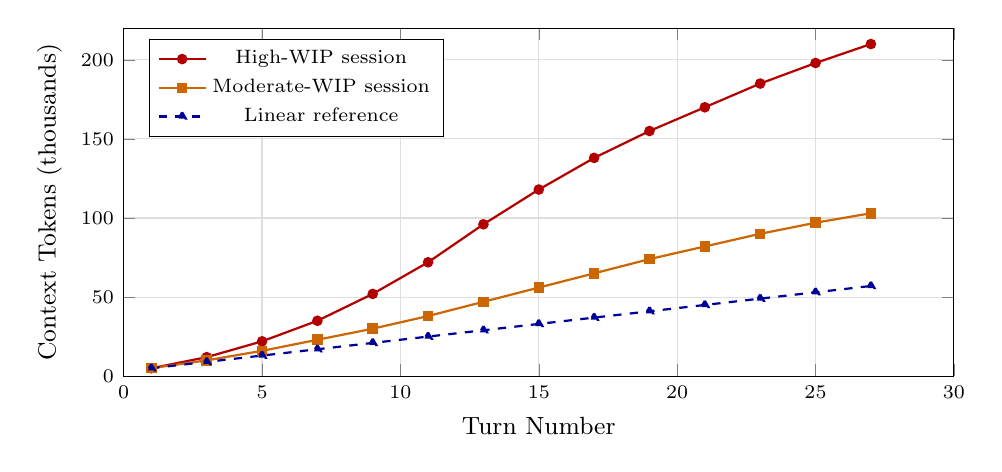
\begin{tikzpicture}
\begin{axis}[
  width=\columnwidth,
  height=6cm,
  xlabel={Turn Number},
  ylabel={Context Tokens (thousands)},
  xmin=0, xmax=30,
  ymin=0, ymax=220,
  grid=major,
  grid style={gray!25},
  tick label style={font=\scriptsize},
  label style={font=\small},
  legend style={font=\scriptsize, at={(0.03,0.97)}, anchor=north west},
]

% Superlinear accumulation curve (high-WIP session)
\addplot[thick, red!70!black, mark=*, mark size=1.5pt] coordinates {
  (1, 5) (3, 12) (5, 22) (7, 35) (9, 52)
  (11, 72) (13, 96) (15, 118) (17, 138)
  (19, 155) (21, 170) (23, 185) (25, 198) (27, 210)
};
\addlegendentry{High-WIP session}

% Moderate growth curve
\addplot[thick, orange!80!black, mark=square*, mark size=1.5pt] coordinates {
  (1, 5) (3, 10) (5, 16) (7, 23) (9, 30)
  (11, 38) (13, 47) (15, 56) (17, 65)
  (19, 74) (21, 82) (23, 90) (25, 97) (27, 103)
};
\addlegendentry{Moderate-WIP session}

% Linear reference (ideal)
\addplot[thick, blue!60!black, dashed, mark=triangle*, mark size=1.5pt] coordinates {
  (1, 5) (3, 9) (5, 13) (7, 17) (9, 21)
  (11, 25) (13, 29) (15, 33) (17, 37)
  (19, 41) (21, 45) (23, 49) (25, 53) (27, 57)
};
\addlegendentry{Linear reference}

\end{axis}
\end{tikzpicture}
\caption{Illustrative context-accumulation trajectories over session turns. The high-WIP trajectory shows superlinear growth relative to the linear reference. Little's Law motivates the WIP accounting relation; the curvature itself is interpreted as an empirical saturation/queueing pattern rather than as a direct prediction of Little's Law.}
\label{fig:context_accumulation}
\end{figure}

\subsection{Semantic Yield}

Having demonstrated the divergence between waste purity and flow efficiency, the analysis now turns to a complementary dimension: the information content of the output itself. Table~\ref{tab:info_throughput} presents Semantic Yield and its components for representative sessions. The data expose a pattern that neither TER nor TFE captures: \emph{information density varies inversely with session size}.

\begin{table}[t]
\centering
\caption{Semantic Yield Across Session Sizes}
\label{tab:info_throughput}
\begin{tabular}{@{}lrrrr@{}}
\toprule
\textbf{Session Type} & $n$ & \textbf{Mean} $\sigma_{\text{sem}}$ & \textbf{Mean} $T_{\text{out}}$ & \textbf{Mean IT} \\
\midrule
Agent subprocess      & 10  & 0.671 & 2,139  & 1,435  \\
Small primary ($<$20K) & 4  & 0.548 & 11,562 & 6,336  \\
Medium primary (20--60K) & 7 & 0.501 & 41,892 & 20,988 \\
Large primary ($>$60K)  & 4 & 0.484 & 79,156 & 38,311 \\
\bottomrule
\end{tabular}
\end{table}

Agent subprocesses have the highest mean semantic density (0.671). The mean value decreases for the small, medium, and large primary sessions, and reaches 0.484 for the largest sessions, 28\% below the subprocess mean. This distribution is consistent with the possibility that larger contexts contain more restatement or re-derivation~\cite{liu2024}. However, task scope, difficulty, session role, and session size also differ among the groups and may contribute to the observed pattern.

Total Semantic Yield nevertheless increases with session size. A large primary session produces $26.7\times$ the output tokens of an agent subprocess and, at 72\% of the mean semantic density, yields $19.3\times$ the redundancy-adjusted output. The density gap is therefore an observed association in this sample rather than an estimate of the causal cost of high WIP.

\subsection{Positional Flow Degradation}

For the temporal evolution of flow, positional TER data (early/mid/late session thirds) provides an additional lens through which to examine production dynamics. Across the 9 sessions with measurable waste, the mean positional TER profile exhibits a characteristic pattern:

\begin{itemize}[leftmargin=*, nosep]
  \item \textbf{Early third:} Mean TER 0.873 (high variance, $\sigma = 0.22$)
  \item \textbf{Mid third:} Mean TER 0.952 (moderate variance, $\sigma = 0.17$)
  \item \textbf{Late third:} Mean TER 0.994 (low variance, $\sigma = 0.003$)
\end{itemize}

Interpreted through the flow lens, the early-phase variance reflects \emph{setup time}: that is to say, the token cost of establishing context, orienting to the task, and loading the necessary material. In manufacturing terms, this is changeover time, which Lean prescribes minimising through SMED (Single-Minute Exchange of Die) techniques~\cite{ohno1988}. The late-phase convergence to near-perfect TER, despite context accumulation, suggests that waste in long sessions is not uniformly distributed but rather concentrates in phase transitions and context-loading operations, precisely the non-value-adding steps that VSM is designed to expose. This finding reinforces the argument that flow-level analysis, which examines \emph{where} in the production process inefficiency arises, provides diagnostic visibility that aggregate waste metrics cannot.

\subsection{Subprocesses as an Observational Analogue of Single-Piece Flow}

The 10 agent subprocesses provide an observational comparison with the 15 primary sessions and can be viewed as an analogue of single-piece flow versus batch processing. In manufacturing, single-piece flow, processing one item at a time through all stages before starting the next, minimises WIP, reduces lead time, and exposes quality problems immediately~\cite{ohno1988}.

Agent subprocesses provide an analogue of single-piece flow: each receives a narrow, scoped task and returns a result to a parent workflow. Primary sessions are more batch-like because multiple tasks, evolving intent, and context can accumulate within one production run. This is an architectural comparison rather than a randomised treatment.

\begin{table}[t]
\centering
\caption{Single-Piece Flow (Subprocesses) vs.\ Batch (Primary Sessions)}
\label{tab:flow_comparison}
\begin{tabular}{@{}lrr@{}}
\toprule
\textbf{Metric} & \textbf{Subprocesses} & \textbf{Primary Sessions} \\
\midrule
Mean TER              & 1.000  & 0.978  \\
Mean TFE              & 0.031  & 0.003  \\
Mean CV               & 12,450 & 5,876  \\
Mean $\sigma_{\text{sem}}$ & 0.671 & 0.509 \\
Mean WIP$_R$          & 0.52   & 0.97   \\
Context bloat rate    & 0\%    & 27\%   \\
Superlinear growth    & 0\%    & 40\%   \\
\bottomrule
\end{tabular}
\end{table}

Table~\ref{tab:flow_comparison} shows large descriptive differences: subprocesses have $10\times$ higher mean TFE, $2.1\times$ higher context velocity, 32\% higher mean semantic density, and a lower WIP ratio. No subprocess in the sample exhibits context bloat or superlinear growth, compared with 27\% and 40\%, respectively, among primary sessions. These directions are consistent with Lean's single-piece-flow expectations~\cite{reinertsen2009, poppendieck2003}, but task scope and session role are confounded with subprocess status; the comparison does not identify a causal effect of decomposition.

The implication is not that all work should be decomposed into subprocesses; some tasks require the sustained context that only a long session provides~\cite{barke2023}. The flow data do suggest, however, that monolithic sessions which accumulate multiple tasks and growing context may be flow-inefficient in some settings. A hybrid architecture (short, scoped subprocesses for discrete tasks, orchestrated by a lightweight parent session that manages intent and context) would better align with Lean's flow principles, and it is towards such an architecture that the recommendations in the concluding section are directed.

% ============================================================================
\section{Discussion}
\label{sec:discussion}

\subsection{Flow Complements Waste}

Our results show that TER and TFE describe different properties of the token production system. TER is a \emph{product metric}~\cite{fenton2014}: it measures the quality (purity) of the output. TFE, by contrast, is a \emph{process metric}: it measures how efficiently the production system converts its total resource consumption into value. The 196--720$\times$ divergence between TER and TFE (Table~\ref{tab:tfe_vs_ter}, Fig.~\ref{fig:ter_tfe_divergence}) quantifies a large difference between output purity and the aligned-output share of counted token traffic. Under the present TFE denominator, this is the strongest empirical motivation for treating flow as a complementary analytical lens; its absolute magnitude should be interpreted together with the denominator choice described in Section~\ref{sec:model}.

This distinction is important in practice. An organisation optimising for TER alone might conclude that its AI coding sessions are highly efficient (mean TER 0.987), while the present TFE accounting indicates that less than 0.4\% of counted token traffic forms value-adding output. The remaining share is dominated by context loading, cache traffic, and input token accumulation under the chosen denominator. Lean's contribution, one that transfers directly to this domain, is the recognition that both views are necessary~\cite{womack1996}: product quality and process efficiency are complementary, not substitutable, and an organisation that attends to only one does so at the cost of systematic blindness to the other.

\subsection{Towards Pull-Based Token Production}

The Token Value Stream Map (Fig.~\ref{fig:vsm}) indicates that the three central phases of the process are predominantly push-driven after the initial developer request. Pull is reintroduced mainly during review and integration. Lean studies show that pull mechanisms can limit WIP and stabilise production~\cite{hopp2004, anderson2010}. For AI coding agents, similar controls would have to act during an otherwise largely autonomous session.

We identify three possible intervention points. First, \emph{reasoning budget controls}, adaptive token budgets~\cite{selfbudgeter2025, tale2024, routetoreason2025} that limit reasoning production based on task complexity, introduce a demand signal into Phase~2. Second, \emph{intent-driven tool selection}, whereby tool invocations are constrained by explicit intent alignment rather than model autonomy, converts Phase~3 from push to pull. Third, \emph{real-time developer feedback}, mechanisms by which the developer can signal ``enough'' mid-session without terminating the session entirely, introduces continuous pull into Phase~4.

\subsection{WIP Limits for Context Windows}

Table~\ref{tab:wip_regimes} suggests that higher input-growth sessions in this sample have lower flow metrics and more context-bloat indicators. The boundaries at 3 and 10 are descriptive bins, not validated operating limits, so the data do not justify a universal ``efficient regime'' or a direct mapping from context growth to server-utilisation thresholds. Queueing theory~\cite{kleinrock1975} nevertheless provides a useful interpretive analogy for why growing inventories can coincide with nonlinear delay or congestion. This motivates---but does not validate---candidate controls such as context budgets, summarisation triggers, and session-splitting heuristics.

\subsection{Limitations}

The main limitations of this study concern the definition of the metrics, the observational dataset, and the generalisation of the results.

\textbf{Construct validity.} The study-specific semantic density computation ($\sigma_{\text{sem}}$) depends on its embedding model and similarity threshold~\cite{reimers2019}; alternative formulations can change absolute Semantic Yield values. It is a redundancy proxy, not a direct information-theoretic quantity, and it differs from TER v3.0.0's production semantic-density scorer. TFE's denominator includes cache-read tokens, which represent reuse rather than new production; alternative denominator formulations may yield different efficiency characterisations. The absence of wall-clock timing prevents direct computation of temporal takt or lead time.

\textbf{Internal validity.} The dataset comprises sessions from one developer using one tool (Claude Code), without controlled assignment of tasks to primary sessions or subprocesses. Session size, task type, task difficulty, subprocess status, and context growth may therefore be confounded. The observed input-growth-group and semantic-density differences are associations, not causal estimates. The group boundaries were selected visually rather than by a formal change-point procedure. Flow metrics are computed from session-level aggregate data; timestamped per-turn analysis is outside the present dataset.

\textbf{External validity.} Twenty-five sessions from a single developer and codebase may not generalise across tools, developers, or task types. The descriptive WIP-group boundaries ($r_{\text{growth}} < 3$, $\geq 10$) are derived from these 25 observations and should not be treated as thresholds; cross-developer and cross-tool replication is needed to determine whether comparable structure recurs.

Replication with additional developers and tools is required to establish the external validity of these results. With respect to the practical requirements of such replication, three conditions must be met: (1)~alternative AI coding tools (Cursor, GitHub Copilot Chat, Windsurf, and similar agents) must expose per-turn token economics with cache breakdowns, data that is not currently available from all tools; (2)~a diverse developer cohort spanning experience levels, task domains, and coding styles must generate a sufficiently large session corpus; and (3)~the same flow metrics must be applied to the resulting data to test whether the observed input-growth pattern, the TFE--TER divergence, and the subprocess/primary-session differences replicate. the metrics themselves are tool-agnostic (they depend only on token counts and semantic density, not on tool-specific internals) and are therefore directly applicable to any LLM coding agent that exposes session-level economics data. The primary barrier to replication is not methodological but practical: obtaining the requisite token accounting data from tools that do not currently expose it.

% ============================================================================
\section{From Measurement to Action: The TGV System}
\label{sec:tgv}

The flow metrics describe the behaviour of existing sessions but do not by themselves modify the production process. We therefore also describe TGV (Task Gateway and Validator)~\cite{griffin2026tgv}, an open-source routing system in which several of the proposed flow-control ideas can be implemented.

\subsection{Architecture and Design Rationale}

TGV is a local-first gateway that intercepts developer task requests before they reach an AI coding agent, profiles each request for complexity and risk, and routes it to one of four capability tiers: \emph{local\_fast} (simple extractive tasks), \emph{local\_code} (bounded code generation), \emph{frontier\_standard} (ambiguous or repository-aware tasks), and \emph{frontier\_deep} (high-risk, architectural, or security-sensitive work). The routing decision is informed by a deterministic weighted-signal engine that extracts eight features from the request text and scores them against per-route weight matrices, with mandatory safety overrides for high-risk signals~\cite{griffin2026tgv}.

In relation to the flow model, the TGV routing architecture implements two of the pull mechanisms discussed in Section~\ref{sec:discussion}. First, by profiling task complexity \emph{before} production begins, TGV introduces a demand signal into the token production pipeline: simple tasks are routed to lightweight local models that produce minimal context overhead, while complex tasks are directed to frontier models with appropriately scoped context bundles. This pre-production routing forms a form of \emph{workload--capacity matching}, in which the production capacity allocated to a task is proportioned to the task's actual requirements rather than defaulting to a single monolithic production system. Second, TGV's context bundle compiler assembles structured evidence packages (repository search results, symbol extractions, and task profiles) that provide the frontier model with precisely scoped input, targeting the context-assembly overhead highlighted conceptually in the Token Value Stream Map (Fig.~\ref{fig:vsm}).

\subsection{The TER Calibration Loop}

TGV v0.29 integrates with TER-compatible telemetry to calibrate the two local routes, \emph{local\_fast} and \emph{local\_code}~\cite{griffin2026ter, griffin2026tgv}. Once the configured minimum number of sessions is available (default 5), the calibration logic compares each local route's observed waste ratio with a target (default 0.25). It proposes a higher local-routing confidence threshold when waste exceeds the target, holds the threshold when waste lies between half the target and the target, and lowers it when waste is below half the target. These are threshold proposals for local-routing selectivity rather than direct manipulation of context WIP.

From the flow perspective, this calibration loop is a candidate \emph{upstream} control mechanism: it changes which tasks are admitted to local execution based on measured outcomes. The present study does not show that TGV enforces the descriptive $r_{\text{growth}}$ grouping boundaries or reduces WIP causally; that relationship is a design interpretation to be evaluated experimentally.

\subsection{Bayesian Outcome Learning}

TGV also maintains a Bayesian-smoothed routing scoreboard based on previous outcomes for each model, capability tier, and task category. Success probability is estimated via a Beta(1,1) prior, $p = (s+1)/(n+2)$, where $s$ is the number of successful outcomes and $n$ the total sample count. A multi-component utility function aggregates success probability, quality indicators (test passage, static analysis), developer acceptance rate, cost, latency, rework frequency, and safety incident rate into a single expected utility score~\cite{griffin2026tgv}. When sufficient samples have accumulated (a configurable minimum, default 5), the scoreboard's recommendation can override the deterministic routing baseline, thus enabling the system to learn from its own decisions and adapt routing behaviour to the observed characteristics of the specific models and workflows deployed in a given organisation.

This adaptive mechanism avoids hard-coding the manuscript's descriptive WIP boundaries into the router. Instead, TGV can adapt routing recommendations to organisation-specific outcome histories. Whether that adaptation improves the flow metrics proposed here remains an empirical question outside the present observational study.

\subsection{Implications for Flow Theory}

We use TGV as an implementation example rather than as a validation of the flow model. Its context-bundle compiler targets context assembly, which the value-stream model highlights as a candidate source of overhead; its tiered routing matches task scope to model capability; and its TER-informed calibration links post-hoc efficiency measurements to routing-threshold proposals. These mechanisms instantiate several control ideas motivated by the framework, but this paper does not evaluate TGV against a baseline or establish that they improve TFE, CV, or WIP Ratio.

% ============================================================================
\section{Related Work}
\label{sec:related}

TER~\cite{griffin2026ter} supplies the waste-classification baseline that this paper extends with flow-theoretic metrics. The adaptive reasoning literature (SelfBudgeter~\cite{selfbudgeter2025}, TALE~\cite{tale2024}, Route-To-Reason~\cite{routetoreason2025}) addresses token efficiency from the model's perspective, optimising reasoning budgets at inference time. In effect, and as noted in Section~\ref{sec:discussion}, these approaches implement pull mechanisms for Phase~2 (reasoning) of the token value stream, though none frames the contribution in those terms.

On the input side of the value stream, the context engineering literature (LLMLingua-2~\cite{llmlingua2_2024}, Anthropic's context engineering guidance~\cite{anthropic_context2025}) seeks to minimise raw material (input token) consumption. Liu et~al.'s~\cite{liu2024} ``lost in the middle'' finding provides a cognitive mechanism for the flow degradation observed in the empirical analysis presented here: as context WIP accumulates, the model's attention to earlier material degrades, necessitating re-reading (motion waste) and re-derivation (overprocessing waste) that impede flow.

The software engineering flow literature (Anderson~\cite{anderson2010}, Forsgren et~al.~\cite{forsgren2018, forsgren2021}, Reinertsen~\cite{reinertsen2009}) provides the theoretical and empirical foundations that this paper extends to the AI-assisted development domain. Meadows~\cite{meadows2008} offers the systems-thinking perspective that frames the context window as a stock-and-flow system with feedback loops, reinforcing the analytical approach taken here and providing the conceptual vocabulary whereby token production dynamics can be understood as emergent system behaviours rather than isolated inefficiencies.

% ============================================================================
\section{Conclusion}
\label{sec:conclusion}

We have applied Lean flow concepts to the token production process of AI coding agents. In the 25 sessions analysed here, TER values close to one can occur together with TFE values below 0.004. Sessions with larger input growth have lower mean context velocity and more context-bloat indicators, and subprocesses have better mean flow metrics than primary sessions. The latter observations are descriptive and do not demonstrate either a causal effect or a universal threshold.

The results suggest three directions for further tests: explicit controls on context WIP, hybrid architectures using scoped subprocesses, and pull mechanisms such as adaptive reasoning budgets or developer feedback. TGV v0.29 provides one implementation of related ideas through capability-tier routing, TER-informed calibration of local-routing thresholds, and Bayesian outcome learning. Its effect on TFE, CV, or WIP Ratio is not evaluated here. Controlled experiments with different developers, tools, and task types will be needed to determine whether these interventions improve token flow.

\section*{Data Availability}

The product implementations referenced in this manuscript are TER v3.0.0, maintained at \url{https://github.com/lgriffin/TER}, and TGV v0.29, maintained at \url{https://github.com/cplegendre/TGV}. The study-specific semantic-density procedure used for Table~\ref{tab:info_throughput} is distinct from TER v3.0.0's production \texttt{SemanticDensityScorer}; reproducing the reported SY values therefore requires the research pipeline described in Section~\ref{sec:model}, together with the derived session-level semantic-density scores. Raw session transcripts are not distributed because they contain proprietary code content. The session-level token economics, derived semantic-density scores, flow-metric scripts, and WIP-boundary sensitivity analysis represent the manuscript's replication artefacts. A submission-ready release should archive these artefacts with an immutable version identifier (for example, a tagged repository release or archival DOI) so that the reported tables and figures can be reproduced independently of subsequent TER product changes.

\bibliographystyle{IEEEtran}
\bibliography{references}

\end{document}
